% Section of thesis on DUNE 35ton prototype
% Target: 30 pages

\graphicspath{{35ton/Figs/}}

\chapter{The DUNE 35~ton Prototype}\label{chap:35ton}

The 35~ton is a prototype experiment for the DUNE far detector design.  It was contructed to prototype the unique design features of the LBNE far detector and was the only planned prototype for this detector.  Following the dissolution of LBNE and the subsequent merging along with LBNO into the DUNE experiment, the 35~ton has become an integral part of the design and execution of the DUNE far detector design.

The 35~ton consists of a membrane cryostat (Sec. \ref{sec:35tonCryostat}), designed to be filled with 35 metric tons of liquid argon, and a small-scale DUNE-style detector (Sec. \ref{sec:35tonDetector}) including a TPC and photon detectors.  It was constructed in 2012 at PC4, a former proton facility in a decomissioned beamline, at Fermilab.  The Phase I run, without a detector, took place between December 2013 and February 2014.  Between February 2014 and September 2015 the detector was constructed and heavily tested at FNAL before being installed inside the cryostat ready for the Phase II run.  This took place between February 2016 and April 2016 (offically starting on 11th February, as I type!).

%------------------------------------------------------------------------------------------------------------------------------------------------------------
\section{Motivation}\label{sec:35tonMotivation}

The use of liquid argon TPCs (LArTPCs) for the study of neutrinos in long-baseline experiments shows great promise and is the direction neutrino research, particularly in the US, is headed.  Fermilab has an extensive program of LArTPC experiments to design, test and improve such detectors, culminating in DUNE, the flagship experiment due to come online in the early 2020s.  Although they exhibit great physics potential, they do not come without significant engineering challenges.  For example, DUNE will have four 10 kton cryostats containing liquid argon kept at very high purity.  Constructing such a cryostat is itself difficult and expensive but in order to achieve, and maintain, the required purity, much R\&D is required.

Previous LArTPC experiments, such as ICARUS [], Argoneut [], LArIAT [] and MicroBooNE [] (?), have been contructed as flat plane vessels and have used an evacuation method as the first step in removing atmospheric impurities which would contaminate the liquid argon.  Constructing the DUNE far detector cryostats in a similar mannor would be both very expensive and incredibly challenging.  In order to investigate possible alternatives, the Fermilab program includes the Liquid Argon Purity Demonstrator (LAPD) and 35~ton experiments, together showing a cheaper and more feasible approach to designing and operating LArTPCs.  These experiments are the subject of the present chaptor.

%------------------------------------------------------------------------------------------------------------------------------------------------------------
\section{The Liquid Argon Purity Demonstrator}\label{sec:LAPD}

The Liquid Argon Purity Demonstrator (LAPD) \cite{LAPD} was designed to demonstrate that the required purity of future LArTPC experiments is possible to acheive without the use of large scale vacuum pumps.  The required mechanical capability of the cryostat to withstand such a method, along with the operation of the evacuation system itself, adds a considerable amount to the cost of the project.  Suggestions to get around this include using multiple smaller scale cryostats, but this leads to greater complexity relating to both the engineering requirements of the piping infrastructure and the reconstruction capabilities of interactions spanning numerous fiducial volumes.  LAPD successfully pioneered the method of using purging as the first step in purification of the liquid argon.  This important result is discussed below and has significantly influenced the design of future LAr cryostats, including the 35~ton.

\subsection{LAPD Experimental Setup}\label{sec:LAPDExperimentalSetup}

LAPD consists of a cylindrical tank (diameter 10 feet, height 10 feet) with a domed head capable of holding 32.6 tons of liquid argon.  It is instrumented with cryogenic equipment and a purification system, consisting of two purifiers and a piping system.  Figure \ref{fig:LAPDTankPiping} shows a CAD model of the tank and purification piping.

\begin{figure}[ht]
  \centering
  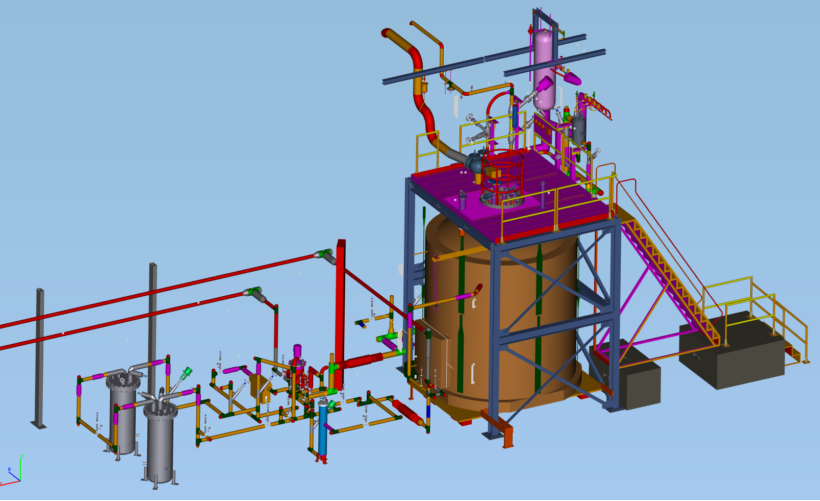
\includegraphics[width=15cm]{LAPDTankPiping.png}
  \caption[LAPD tank and purification system]{The LAPD tank and purification system \cite{LAPD}.  The domed tank on the right, beneath the platform, is the cryostat.  The piping allow the flow of liquid argon into and out of the cryostat and is used as part of the purification system.  Two cylindrical purifiers, visible in the lower left of the figure, remove contaminants from the argon as it is pumped through.  All components of the experiment are discussed in the text.}
  \label{fig:LAPDTankPiping}
\end{figure}

Insulation for the tank is provided by fibreglass sheets covering the outer volume which, along with the tank, is refrigerated by liquid nitrogen from an external supply.  There also exist cooling coils near the top of the tank which serve to recondense vapourised argon and feed it back into the tank, via the filtration system.

The liquid argon is fed into the tank from outside PC4  The argon purity is maintained through the use of the purifiers, located outside of the main volume.  Argon is constantly circulated from the tank to these vessels through stainless steel pipes.  The filtration system used by LAPD, and subsequently by the 35~ton cryostat, is discussed in greater detail in ection \ref{sec:LAPDFiltration}.

\subsection{The LAPD Filtration System}\label{sec:LAPDFiltration}

A LArTPC relies on the detection of the drift electrons produced upon ionisation of the argon by a propagating particle.  Electronegative contaminants in the medium jeopardise this process by recombining with the electrons before they can reach the readout electronics.  The phase `electron lifetime' therefore refers to the amount of time that an electron will typically drift along the electron field, and is directly related to the concentration of impurities in the liquid.  Even using a modularised detector, as the DUNE far detector will be, drift lengths on the order of 5 m are realistically required, leading to purity requirements of several milliseconds.  The dominant contaminents which are removed by the LAPD and 35~ton filtration system are oxygen and water.

The liquid argon is extracted from near the bottom of the tank and returned to the top after passing through the purifiers.  It first passes through the water filter before continuing on through the oxygen filter.  The water filter comprises a molecular sieve which prevents the propagation of large molecules, such as water.  This purification step must occur first since the proceeding filter also removes water molecules and would therefore be less efficient at removing oxygen if used first.  The oxygen filter consists of a thin activated-copper layer on an alumnia substrate \cite{LArFilter}.  Both filters will lose some functionality over time as they collect more and more impurities and so require `regenerating' in order to remove the contaminants.  This can be done in-situ, as described in \cite{LArFilter}; this complicates the design of the filter but is necessary when considering the purification system required for the full DUNE far detector.

The contamination gradient, and associated purities at each stage during the LAPD Phase II run, is shown in figure \ref{fig:LAPDPurity}.  These purities are known through the use of purity monitors; these are the subject of section \ref{sec:PurityMonitoring}.

\begin{figure}[ht]
  \centering
  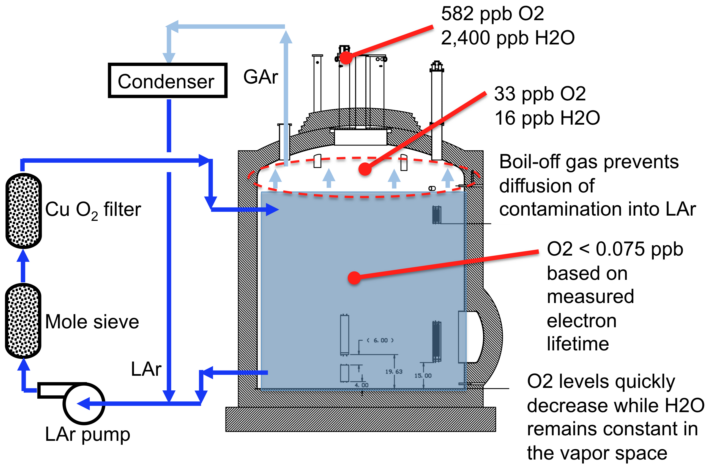
\includegraphics[width=12cm]{LAPDPurity.png}
  \caption[Contaminant gradient in the LAPD tank]{Contaminant gradient in the LAPD tank at different stages of the purification process \cite{LAPD}.  The associated LAr purities, in units of parts-per-billion (ppb) are also shown.}
  \label{fig:LAPDPurity}
\end{figure}

\subsection{Purity Monitoring}\label{sec:PurityMonitoring}

As discussed in section \ref{sec:LAPDFiltration}, extreme LAr purity is required for the successful readout of ionisation electrons by the electronics.  These purites must be constatly monitored to ensure the high quality of argon necessary during data taking.  Since these impurity concentrations on beyond the capabilities of many conventional gas analysers, a device called a purity monitor is employed.  Such a device is shown schematically in figure \ref{fig:PurityMonitor}.

\begin{figure}[ht]
  \centering
  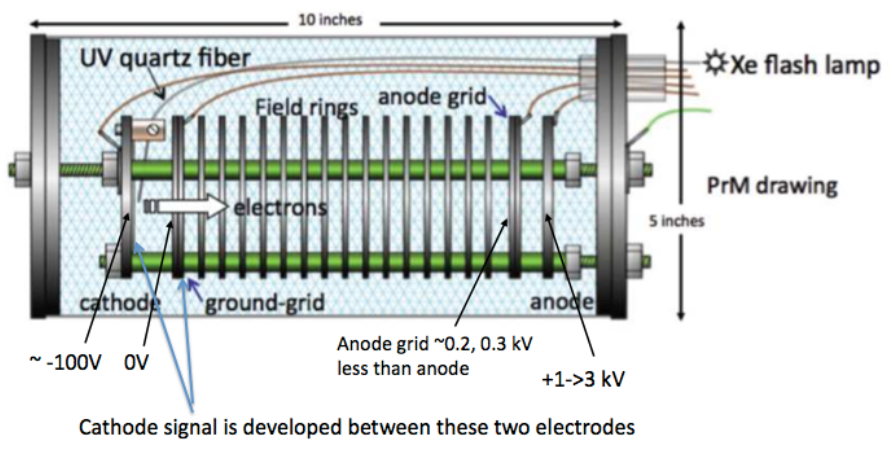
\includegraphics[width=12cm]{PurityMonitor.png}
  \caption[Design of LAPD and 35~ton style purity monitors]{Diagram showing schematically the design of purity monitor used in LAPD, and subsequently the 35~ton experiment \cite{LBNE35tonPhaseI}.  Their use is described in the text.}
  \label{fig:PurityMonitor}
\end{figure}

The purity monitors deployed consist of a cylindrical volume, filled with LAr for its surrounding environment.  They contain a photo cathode and an anode, between which lies short drift volume.  When taking purity measurments, light from a Xenon flash lamp is incident on the cathode, liberating photoelectrons which traverse towards the anode.  Electronegative impurities in the LAr will decrease the electron lifetime and therefore the mean number of electrons reaching a certain point along the drift volume.  A measurement of the ratio of the charge arriving at the anode to that at the cathode is hence a measurement of the inherit purity of the liquid.

These monitors were placed both in the LAPD tank and just after the filtration system in order to study the purity at different points in the recirculation.  Several gas analysers, measuring nitrogen, oxygen and water contaminants to various levels of accuracy, were also used.  Temperature sensors to measure the vertical temperature profile within the cryostat were necessary to account its effect on the electron drift velocity.

Several of the technologies pioneered in LAPD were also used in the 35~ton experiment, as will be shortly discussed.

\subsection{LAPD Results}\label{sec:LAPDResults}

LAPD successfully demonstrated achieving and maintaining the required LAr purity for a large neutrino detector is possible without the costly and challenging use of evacuation techniques.  It initially ran for six weeks and reached a purity of better than 60 ppt (parts-per-trillion) oxygen equivalent \cite{LAPD}.  The measured electron lifetimes over the course of the run is shown in figure \ref{fig:ElectronLifetimes}.  As can be seen, electron lifetimes of up to 4 ms were reached, which is [put into context with current DUNE requirements!].

\begin{figure}[ht]
  \centering
  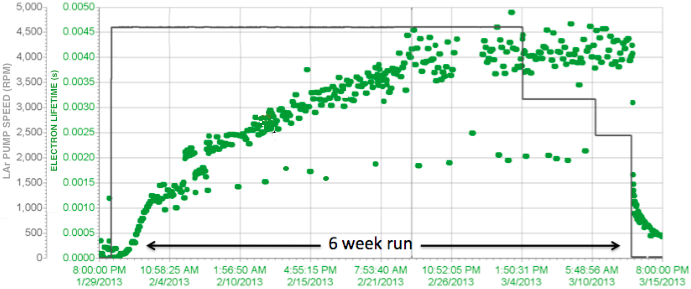
\includegraphics[width=15cm]{LAPDElectronLifetime.png}
  \caption[]{}
  \label{fig:LAPDElectronLifetime}
\end{figure}

This important result has great significance when considering future LArTPC experiments and laid the way for the 35~ton experiment.  This experiment will now be discussed in the subsequent sections.

%------------------------------------------------------------------------------------------------------------------------------------------------------------
\section{The 35~ton Cryostat}\label{sec:35tonCryostat}

The 35~ton prototype takes advantage of membrane cryostat technology and is the first test of this construction technique for LArTPCs.  Membrane cryostats have been widely used in the liquified natural gas industry for many years but the 35~ton experiment is the first to make use of the technology for liquid argon.  Furthermore, it is the first membrane cryostat to be constructed in the United States and the first to be constructed for scientific purposes \cite{LBNE35tonPhaseIOverview}.  The 35~ton cryostat is the subject of the present section.

\subsection{Construction}\label{sec:35tonCryostatConstruction}

Boring stuff about cement and shit.

\begin{figure}[ht]
  \centering
  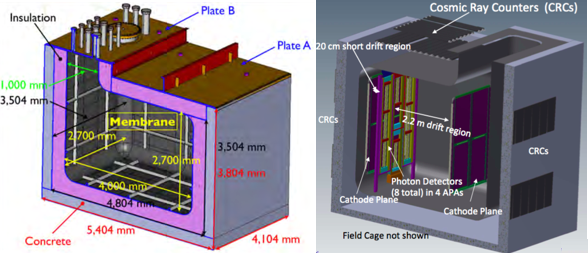
\includegraphics[width=15cm]{35tonCryostat.png}
  \caption[The 35~ton cryostat]{The 35~ton cryostat \cite{LBNE35tonPhaseI}.  The cryostat as operated during Phase I is shown on the left and the corresponding version, including a full small-scale detector, used in Phase II is on the right.}
  \label{fig:35tonCryostat}
\end{figure}

Cryostat!

\subsection{The 35~ton and LAPD}\label{35tonLAPD}

It's near LAPD!

\begin{figure}[ht]
  \centering
  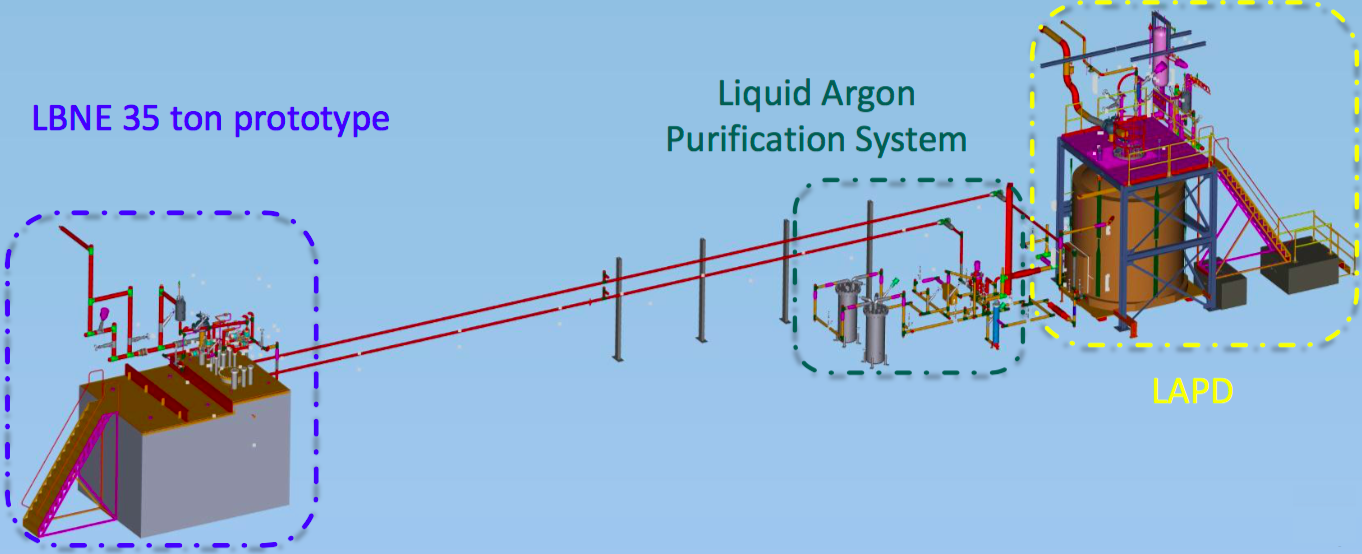
\includegraphics[width=15cm]{35tonLAPD.png}
  \caption[]{\cite{LBNE35tonPhaseI}.}
  \label{fig:35tonLAPD}
\end{figure}

%------------------------------------------------------------------------------------------------------------------------------------------------------------
\section{The 35~ton Detector}\label{sec:35tonDetector}

\subsection{Detector Components}\label{sec:35tonDetectorComponents}

\subsubsection{TPC}\label{35tonTPC}

\subsubsection{Photon Detectors}\label{35tonPhoton}

\subsubsection{External Counters}\label{35tonCounters}

\subsection{Readout Electronics}\label{sec:35tonReadoutElectronics}

\subsubsection{FEMBs}\label{35tonFEMB}

\subsubsection{RCEs}\label{35tonRCE}

\subsubsection{SSPs}\label{35tonSSP}

\subsubsection{PTB}\label{35tonPTB}

\subsection{DAQ}\label{35tonDAQ}

%------------------------------------------------------------------------------------------------------------------------------------------------------------
\section{Filling the 35~ton}\label{sec:35tonFilling}

%------------------------------------------------------------------------------------------------------------------------------------------------------------
\section{The 35~ton Experimental Setup}\label{sec:35tonExperiment}

\subsection{Filtration System}\label{sec:35tonFiltration}

Same as LAPD.

\subsection{Purity Monitoring}\label{sec:35tonPurity}

Same as LAPD.

%------------------------------------------------------------------------------------------------------------------------------------------------------------
\section{35~ton Phase I}\label{sec:35tonPhaseI}

\subsection{Outcomes}\label{sec:35tonPhaseIOutcomes}

%------------------------------------------------------------------------------------------------------------------------------------------------------------
\section{35~ton Phase II}\label{sec:35tonPhaseII}

\subsection{Commissioning}\label{sec:35tonCommissioning}

\subsection{The Sheffield Camera System}\label{sec:35tonCameraSystem}

Wait for Nicola to finish the paper and plagerise!

\subsection{Online Monitoring for Data Quality Monitoring}\label{sec:35tonOnlineMonitoring}

\subsection{Outcomes}\label{sec:35tonPhaseIIOutcomes}
































% The very first part of my thesis, written June 2015.  I'll leave it here to remember it!

%% \section{The DUNE 35ton LAr Prototype}

%% The DUNE far detector (see section
%% %\ref{sec:DUNEFD})
%% has a very large, complicated design including many features which are novel to this experiment. In order to optimise and minimise potential complications during construction an\
%% d commissioning, several levels of prototyping are necessary during the design. These include the membrane cryostat, a TPC within such a cryostat, full scale detector elements, \
%% installation test and complete vertical slice tests of all electronics. Many of these have been tested with the first of two DUNE prototypes, the 35-ton (ref Far Detector Extern\
%% al Review, May 19-20 2015).

%% There was a phase 1 run! \cite{LBNE35tonPhase1}

%% \subsection{Overview of the 35-ton}

%% The 35-ton is a
